\documentclass[11pt]{article}
\usepackage[T1]{fontenc}
\usepackage{lmodern}
\usepackage[margin=2.5cm]{geometry}
\usepackage{amsmath,amssymb}
\usepackage{graphicx}
\usepackage{booktabs}
\usepackage{setspace}
\usepackage[numbers,sort&compress]{natbib}
\usepackage[hidelinks]{hyperref}
\usepackage{xurl}
\usepackage{lineno}
\setstretch{1.4}
\emergencystretch=2em
% generated by code/make_macros.py -- do not edit
\makeatletter
\expandafter\def\csname res@aFivebelowACI\endcsname{1}
\expandafter\def\csname res@aFivebelowEMP\endcsname{7}
\expandafter\def\csname res@aFivebelowSCD\endcsname{4}
\expandafter\def\csname res@aFivecovACAMax\endcsname{1.000}
\expandafter\def\csname res@aFivecovACAMin\endcsname{0.999}
\expandafter\def\csname res@aFivecovACIMax\endcsname{0.955}
\expandafter\def\csname res@aFivecovACIMin\endcsname{0.949}
\expandafter\def\csname res@aFivecovEMPMax\endcsname{0.943}
\expandafter\def\csname res@aFivecovEMPMin\endcsname{0.902}
\expandafter\def\csname res@aFivecovMOLMax\endcsname{0.800}
\expandafter\def\csname res@aFivecovMOLMin\endcsname{0.445}
\expandafter\def\csname res@aFivecovSCDMax\endcsname{0.952}
\expandafter\def\csname res@aFivecovSCDMin\endcsname{0.927}
\expandafter\def\csname res@aFiverelACAMax\endcsname{1.92}
\expandafter\def\csname res@aFiverelACAMin\endcsname{1.32}
\expandafter\def\csname res@aFiverelACIMax\endcsname{1.07}
\expandafter\def\csname res@aFiverelACIMin\endcsname{1.03}
\expandafter\def\csname res@aFiverelEMPMax\endcsname{1.03}
\expandafter\def\csname res@aFiverelEMPMin\endcsname{1.00}
\expandafter\def\csname res@aFiverelMOLMax\endcsname{0.95}
\expandafter\def\csname res@aFiverelMOLMin\endcsname{0.89}
\expandafter\def\csname res@aFiverelSCDMax\endcsname{1.07}
\expandafter\def\csname res@aFiverelSCDMin\endcsname{1.02}
\expandafter\def\csname res@aTwentybelowACI\endcsname{2}
\expandafter\def\csname res@aTwentybelowEMP\endcsname{7}
\expandafter\def\csname res@aTwentybelowSCD\endcsname{4}
\expandafter\def\csname res@aTwentycovACAMax\endcsname{1.000}
\expandafter\def\csname res@aTwentycovACAMin\endcsname{0.998}
\expandafter\def\csname res@aTwentycovACIMax\endcsname{0.812}
\expandafter\def\csname res@aTwentycovACIMin\endcsname{0.793}
\expandafter\def\csname res@aTwentycovEMPMax\endcsname{0.789}
\expandafter\def\csname res@aTwentycovEMPMin\endcsname{0.754}
\expandafter\def\csname res@aTwentycovMOLMax\endcsname{0.800}
\expandafter\def\csname res@aTwentycovMOLMin\endcsname{0.445}
\expandafter\def\csname res@aTwentycovSCDMax\endcsname{0.820}
\expandafter\def\csname res@aTwentycovSCDMin\endcsname{0.770}
\expandafter\def\csname res@aTwentyrelACAMax\endcsname{1.91}
\expandafter\def\csname res@aTwentyrelACAMin\endcsname{1.26}
\expandafter\def\csname res@aTwentyrelACIMax\endcsname{1.03}
\expandafter\def\csname res@aTwentyrelACIMin\endcsname{1.01}
\expandafter\def\csname res@aTwentyrelEMPMax\endcsname{1.02}
\expandafter\def\csname res@aTwentyrelEMPMin\endcsname{0.99}
\expandafter\def\csname res@aTwentyrelMOLMax\endcsname{1.01}
\expandafter\def\csname res@aTwentyrelMOLMin\endcsname{0.94}
\expandafter\def\csname res@aTwentyrelSCDMax\endcsname{1.03}
\expandafter\def\csname res@aTwentyrelSCDMin\endcsname{1.01}
\expandafter\def\csname res@acaOverMOLMax\endcsname{107}
\expandafter\def\csname res@acaOverMOLMin\endcsname{40}
\expandafter\def\csname res@acaOverSCDMax\endcsname{84}
\expandafter\def\csname res@acaOverSCDMin\endcsname{27}
\expandafter\def\csname res@aciOverSCDMax\endcsname{1.0}
\expandafter\def\csname res@aciOverSCDMin\endcsname{0.0}
\expandafter\def\csname res@aciSig\endcsname{3}
\expandafter\def\csname res@aciSigNames\endcsname{the Bronx, Queens and Brooklyn}
\expandafter\def\csname res@aciSigPMax\endcsname{0.027}
\expandafter\def\csname res@areaName\endcsname{Q4}
\expandafter\def\csname res@belowACAArea\endcsname{0}
\expandafter\def\csname res@belowACABK\endcsname{0}
\expandafter\def\csname res@belowACABX\endcsname{0}
\expandafter\def\csname res@belowACAMN\endcsname{0}
\expandafter\def\csname res@belowACAMax\endcsname{0}
\expandafter\def\csname res@belowACAMin\endcsname{0}
\expandafter\def\csname res@belowACAQN\endcsname{0}
\expandafter\def\csname res@belowACASF\endcsname{0}
\expandafter\def\csname res@belowACASI\endcsname{0}
\expandafter\def\csname res@belowACIArea\endcsname{7}
\expandafter\def\csname res@belowACIBK\endcsname{7}
\expandafter\def\csname res@belowACIBX\endcsname{10}
\expandafter\def\csname res@belowACIMN\endcsname{7}
\expandafter\def\csname res@belowACIMax\endcsname{12}
\expandafter\def\csname res@belowACIMin\endcsname{5}
\expandafter\def\csname res@belowACIQN\endcsname{7}
\expandafter\def\csname res@belowACISF\endcsname{5}
\expandafter\def\csname res@belowACISI\endcsname{12}
\expandafter\def\csname res@belowEMPArea\endcsname{5}
\expandafter\def\csname res@belowEMPBK\endcsname{15}
\expandafter\def\csname res@belowEMPBX\endcsname{20}
\expandafter\def\csname res@belowEMPMN\endcsname{15}
\expandafter\def\csname res@belowEMPMax\endcsname{20}
\expandafter\def\csname res@belowEMPMin\endcsname{5}
\expandafter\def\csname res@belowEMPQN\endcsname{17}
\expandafter\def\csname res@belowEMPSF\endcsname{7}
\expandafter\def\csname res@belowEMPSI\endcsname{10}
\expandafter\def\csname res@belowMOLArea\endcsname{46}
\expandafter\def\csname res@belowMOLBK\endcsname{90}
\expandafter\def\csname res@belowMOLBX\endcsname{71}
\expandafter\def\csname res@belowMOLMN\endcsname{78}
\expandafter\def\csname res@belowMOLMax\endcsname{90}
\expandafter\def\csname res@belowMOLMin\endcsname{27}
\expandafter\def\csname res@belowMOLQN\endcsname{78}
\expandafter\def\csname res@belowMOLSF\endcsname{27}
\expandafter\def\csname res@belowMOLSI\endcsname{59}
\expandafter\def\csname res@belowORArea\endcsname{0}
\expandafter\def\csname res@belowORBK\endcsname{0}
\expandafter\def\csname res@belowORBX\endcsname{0}
\expandafter\def\csname res@belowORMN\endcsname{0}
\expandafter\def\csname res@belowORMax\endcsname{0}
\expandafter\def\csname res@belowORMin\endcsname{0}
\expandafter\def\csname res@belowORQN\endcsname{0}
\expandafter\def\csname res@belowORSF\endcsname{0}
\expandafter\def\csname res@belowORSI\endcsname{0}
\expandafter\def\csname res@belowSCDArea\endcsname{7}
\expandafter\def\csname res@belowSCDBK\endcsname{10}
\expandafter\def\csname res@belowSCDBX\endcsname{12}
\expandafter\def\csname res@belowSCDMN\endcsname{7}
\expandafter\def\csname res@belowSCDMax\endcsname{12}
\expandafter\def\csname res@belowSCDMin\endcsname{5}
\expandafter\def\csname res@belowSCDQN\endcsname{12}
\expandafter\def\csname res@belowSCDSF\endcsname{5}
\expandafter\def\csname res@belowSCDSI\endcsname{12}
\expandafter\def\csname res@belowSIPPArea\endcsname{54}
\expandafter\def\csname res@belowSIPPBK\endcsname{95}
\expandafter\def\csname res@belowSIPPBX\endcsname{88}
\expandafter\def\csname res@belowSIPPMN\endcsname{88}
\expandafter\def\csname res@belowSIPPMax\endcsname{95}
\expandafter\def\csname res@belowSIPPMin\endcsname{32}
\expandafter\def\csname res@belowSIPPQN\endcsname{83}
\expandafter\def\csname res@belowSIPPSF\endcsname{32}
\expandafter\def\csname res@belowSIPPSI\endcsname{63}
\expandafter\def\csname res@bkLoMax\endcsname{0.851}
\expandafter\def\csname res@bkLoMin\endcsname{0.849}
\expandafter\def\csname res@callsArea\endcsname{83}
\expandafter\def\csname res@callsBK\endcsname{1,225}
\expandafter\def\csname res@callsBX\endcsname{1,036}
\expandafter\def\csname res@callsMN\endcsname{1,074}
\expandafter\def\csname res@callsMax\endcsname{1,225}
\expandafter\def\csname res@callsMin\endcsname{83}
\expandafter\def\csname res@callsQN\endcsname{905}
\expandafter\def\csname res@callsSF\endcsname{270}
\expandafter\def\csname res@callsSI\endcsname{192}
\expandafter\def\csname res@carryBK\endcsname{32}
\expandafter\def\csname res@carryMax\endcsname{32}
\expandafter\def\csname res@carryMin\endcsname{2}
\expandafter\def\csname res@condBelowObs\endcsname{9.4}
\expandafter\def\csname res@condBelowTh\endcsname{3.1}
\expandafter\def\csname res@condMeanTh\endcsname{0.902}
\expandafter\def\csname res@condSdObs\endcsname{0.110}
\expandafter\def\csname res@condSdTh\endcsname{0.080}
\expandafter\def\csname res@covACAArea\endcsname{1.000}
\expandafter\def\csname res@covACABK\endcsname{1.000}
\expandafter\def\csname res@covACABX\endcsname{0.999}
\expandafter\def\csname res@covACAMN\endcsname{1.000}
\expandafter\def\csname res@covACAMax\endcsname{1.000}
\expandafter\def\csname res@covACAMin\endcsname{0.999}
\expandafter\def\csname res@covACAQN\endcsname{1.000}
\expandafter\def\csname res@covACASF\endcsname{1.000}
\expandafter\def\csname res@covACASI\endcsname{1.000}
\expandafter\def\csname res@covACIArea\endcsname{0.905}
\expandafter\def\csname res@covACIBK\endcsname{0.902}
\expandafter\def\csname res@covACIBX\endcsname{0.896}
\expandafter\def\csname res@covACIMN\endcsname{0.909}
\expandafter\def\csname res@covACIMax\endcsname{0.909}
\expandafter\def\csname res@covACIMin\endcsname{0.896}
\expandafter\def\csname res@covACIQN\endcsname{0.899}
\expandafter\def\csname res@covACISF\endcsname{0.906}
\expandafter\def\csname res@covACISI\endcsname{0.901}
\expandafter\def\csname res@covEMPArea\endcsname{0.880}
\expandafter\def\csname res@covEMPBK\endcsname{0.845}
\expandafter\def\csname res@covEMPBX\endcsname{0.852}
\expandafter\def\csname res@covEMPMN\endcsname{0.878}
\expandafter\def\csname res@covEMPMax\endcsname{0.890}
\expandafter\def\csname res@covEMPMin\endcsname{0.845}
\expandafter\def\csname res@covEMPQN\endcsname{0.863}
\expandafter\def\csname res@covEMPSF\endcsname{0.890}
\expandafter\def\csname res@covEMPSI\endcsname{0.879}
\expandafter\def\csname res@covLoadDown\endcsname{0.961}
\expandafter\def\csname res@covLoadFlat\endcsname{0.897}
\expandafter\def\csname res@covLoadUp\endcsname{0.801}
\expandafter\def\csname res@covMOLArea\endcsname{0.737}
\expandafter\def\csname res@covMOLBK\endcsname{0.445}
\expandafter\def\csname res@covMOLBX\endcsname{0.559}
\expandafter\def\csname res@covMOLMN\endcsname{0.544}
\expandafter\def\csname res@covMOLMax\endcsname{0.800}
\expandafter\def\csname res@covMOLMin\endcsname{0.445}
\expandafter\def\csname res@covMOLQN\endcsname{0.501}
\expandafter\def\csname res@covMOLSF\endcsname{0.800}
\expandafter\def\csname res@covMOLSI\endcsname{0.656}
\expandafter\def\csname res@covORArea\endcsname{0.905}
\expandafter\def\csname res@covORBK\endcsname{0.904}
\expandafter\def\csname res@covORBX\endcsname{0.909}
\expandafter\def\csname res@covORMN\endcsname{0.906}
\expandafter\def\csname res@covORMax\endcsname{0.909}
\expandafter\def\csname res@covORMin\endcsname{0.902}
\expandafter\def\csname res@covORQN\endcsname{0.906}
\expandafter\def\csname res@covORSF\endcsname{0.904}
\expandafter\def\csname res@covORSI\endcsname{0.902}
\expandafter\def\csname res@covSCDArea\endcsname{0.905}
\expandafter\def\csname res@covSCDBK\endcsname{0.879}
\expandafter\def\csname res@covSCDBX\endcsname{0.880}
\expandafter\def\csname res@covSCDMN\endcsname{0.906}
\expandafter\def\csname res@covSCDMax\endcsname{0.906}
\expandafter\def\csname res@covSCDMin\endcsname{0.876}
\expandafter\def\csname res@covSCDQN\endcsname{0.876}
\expandafter\def\csname res@covSCDSF\endcsname{0.896}
\expandafter\def\csname res@covSCDSI\endcsname{0.896}
\expandafter\def\csname res@covSIPPArea\endcsname{0.718}
\expandafter\def\csname res@covSIPPBK\endcsname{0.389}
\expandafter\def\csname res@covSIPPBX\endcsname{0.474}
\expandafter\def\csname res@covSIPPMN\endcsname{0.462}
\expandafter\def\csname res@covSIPPMax\endcsname{0.771}
\expandafter\def\csname res@covSIPPMin\endcsname{0.389}
\expandafter\def\csname res@covSIPPQN\endcsname{0.456}
\expandafter\def\csname res@covSIPPSF\endcsname{0.771}
\expandafter\def\csname res@covSIPPSI\endcsname{0.628}
\expandafter\def\csname res@dispArea\endcsname{1.4}
\expandafter\def\csname res@dispBK\endcsname{4.6}
\expandafter\def\csname res@dispBX\endcsname{3.0}
\expandafter\def\csname res@dispMN\endcsname{5.2}
\expandafter\def\csname res@dispMax\endcsname{5.2}
\expandafter\def\csname res@dispMin\endcsname{1.4}
\expandafter\def\csname res@dispQN\endcsname{4.2}
\expandafter\def\csname res@dispSF\endcsname{2.7}
\expandafter\def\csname res@dispSI\endcsname{1.8}
\expandafter\def\csname res@empBelowScd\endcsname{7}
\expandafter\def\csname res@extraMOLArea\endcsname{13}
\expandafter\def\csname res@extraMOLBK\endcsname{10}
\expandafter\def\csname res@extraMOLBX\endcsname{8}
\expandafter\def\csname res@extraMOLMN\endcsname{9}
\expandafter\def\csname res@extraMOLMax\endcsname{13}
\expandafter\def\csname res@extraMOLMin\endcsname{5}
\expandafter\def\csname res@extraMOLQN\endcsname{11}
\expandafter\def\csname res@extraMOLSF\endcsname{5}
\expandafter\def\csname res@extraMOLSI\endcsname{12}
\expandafter\def\csname res@extraORArea\endcsname{0.4}
\expandafter\def\csname res@extraORBK\endcsname{1.1}
\expandafter\def\csname res@extraORBX\endcsname{1.1}
\expandafter\def\csname res@extraORMN\endcsname{1.3}
\expandafter\def\csname res@extraORQN\endcsname{1.2}
\expandafter\def\csname res@extraORSF\endcsname{0.5}
\expandafter\def\csname res@extraORSI\endcsname{0.6}
\expandafter\def\csname res@firstTest\endcsname{2022-08-22}
\expandafter\def\csname res@flagsAll\endcsname{0}
\expandafter\def\csname res@fracAACAArea\endcsname{0.0}
\expandafter\def\csname res@fracAACABK\endcsname{0.0}
\expandafter\def\csname res@fracAACABX\endcsname{0.0}
\expandafter\def\csname res@fracAACAMN\endcsname{0.0}
\expandafter\def\csname res@fracAACAQN\endcsname{0.0}
\expandafter\def\csname res@fracAACASF\endcsname{0.0}
\expandafter\def\csname res@fracAACASI\endcsname{0.0}
\expandafter\def\csname res@fracAACIArea\endcsname{1.5}
\expandafter\def\csname res@fracAACIBK\endcsname{1.7}
\expandafter\def\csname res@fracAACIBX\endcsname{1.9}
\expandafter\def\csname res@fracAACIMN\endcsname{1.6}
\expandafter\def\csname res@fracAACIQN\endcsname{1.7}
\expandafter\def\csname res@fracAACISF\endcsname{1.7}
\expandafter\def\csname res@fracAACISI\endcsname{1.6}
\expandafter\def\csname res@fracAEMPArea\endcsname{1.8}
\expandafter\def\csname res@fracAEMPBK\endcsname{2.5}
\expandafter\def\csname res@fracAEMPBX\endcsname{2.4}
\expandafter\def\csname res@fracAEMPMN\endcsname{2.0}
\expandafter\def\csname res@fracAEMPQN\endcsname{2.3}
\expandafter\def\csname res@fracAEMPSF\endcsname{1.9}
\expandafter\def\csname res@fracAEMPSI\endcsname{2.0}
\expandafter\def\csname res@fracAMOLArea\endcsname{3.9}
\expandafter\def\csname res@fracAMOLBK\endcsname{10.0}
\expandafter\def\csname res@fracAMOLBX\endcsname{7.1}
\expandafter\def\csname res@fracAMOLMN\endcsname{6.6}
\expandafter\def\csname res@fracAMOLQN\endcsname{9.2}
\expandafter\def\csname res@fracAMOLSF\endcsname{2.9}
\expandafter\def\csname res@fracAMOLSI\endcsname{4.9}
\expandafter\def\csname res@fracAORArea\endcsname{1.8}
\expandafter\def\csname res@fracAORBK\endcsname{2.0}
\expandafter\def\csname res@fracAORBX\endcsname{2.1}
\expandafter\def\csname res@fracAORMN\endcsname{2.1}
\expandafter\def\csname res@fracAORQN\endcsname{1.9}
\expandafter\def\csname res@fracAORSF\endcsname{1.9}
\expandafter\def\csname res@fracAORSI\endcsname{2.0}
\expandafter\def\csname res@fracASCDArea\endcsname{1.5}
\expandafter\def\csname res@fracASCDBK\endcsname{2.0}
\expandafter\def\csname res@fracASCDBX\endcsname{2.1}
\expandafter\def\csname res@fracASCDMN\endcsname{1.7}
\expandafter\def\csname res@fracASCDQN\endcsname{2.0}
\expandafter\def\csname res@fracASCDSF\endcsname{1.8}
\expandafter\def\csname res@fracASCDSI\endcsname{1.7}
\expandafter\def\csname res@fracASIPPArea\endcsname{4.2}
\expandafter\def\csname res@fracASIPPBK\endcsname{12.0}
\expandafter\def\csname res@fracASIPPBX\endcsname{8.9}
\expandafter\def\csname res@fracASIPPMN\endcsname{8.9}
\expandafter\def\csname res@fracASIPPQN\endcsname{11.0}
\expandafter\def\csname res@fracASIPPSF\endcsname{3.4}
\expandafter\def\csname res@fracASIPPSI\endcsname{5.3}
\expandafter\def\csname res@gOthercovMax\endcsname{0.907}
\expandafter\def\csname res@gOthercovMin\endcsname{0.894}
\expandafter\def\csname res@hFourCircP\endcsname{0.0001}
\expandafter\def\csname res@hFourP\endcsname{0.0001}
\expandafter\def\csname res@hFourRho\endcsname{-0.57}
\expandafter\def\csname res@hFourWithinMax\endcsname{-0.39}
\expandafter\def\csname res@hFourWithinMin\endcsname{-0.69}
\expandafter\def\csname res@hOneFail\endcsname{BX, QN}
\expandafter\def\csname res@hOneLoArea\endcsname{0.885}
\expandafter\def\csname res@hOneLoBK\endcsname{0.850}
\expandafter\def\csname res@hOneLoBX\endcsname{0.841}
\expandafter\def\csname res@hOneLoMN\endcsname{0.880}
\expandafter\def\csname res@hOneLoMax\endcsname{0.885}
\expandafter\def\csname res@hOneLoMin\endcsname{0.841}
\expandafter\def\csname res@hOneLoQN\endcsname{0.844}
\expandafter\def\csname res@hOneLoSF\endcsname{0.861}
\expandafter\def\csname res@hOneLoSI\endcsname{0.870}
\expandafter\def\csname res@hOneNoQMax\endcsname{4}
\expandafter\def\csname res@hOneNoQMin\endcsname{3}
\expandafter\def\csname res@hOneOk\endcsname{5}
\expandafter\def\csname res@hOneSeedMax\endcsname{5}
\expandafter\def\csname res@hOneSeedMin\endcsname{4}
\expandafter\def\csname res@hOneSeedShareMax\endcsname{56}
\expandafter\def\csname res@hThreePMax\endcsname{8.5e-8}
\expandafter\def\csname res@hThreeSig\endcsname{7}
\expandafter\def\csname res@hTwoHolmMin\endcsname{0.079}
\expandafter\def\csname res@hTwoPMax\endcsname{0.16}
\expandafter\def\csname res@hTwoPMin\endcsname{0.011}
\expandafter\def\csname res@hTwoSig\endcsname{0}
\expandafter\def\csname res@hiACAArea\endcsname{1.000}
\expandafter\def\csname res@hiACABK\endcsname{1.000}
\expandafter\def\csname res@hiACABX\endcsname{1.000}
\expandafter\def\csname res@hiACAMN\endcsname{1.000}
\expandafter\def\csname res@hiACAQN\endcsname{1.000}
\expandafter\def\csname res@hiACASF\endcsname{1.000}
\expandafter\def\csname res@hiACASI\endcsname{1.000}
\expandafter\def\csname res@hiACIArea\endcsname{0.928}
\expandafter\def\csname res@hiACIBK\endcsname{0.926}
\expandafter\def\csname res@hiACIBX\endcsname{0.929}
\expandafter\def\csname res@hiACIMN\endcsname{0.933}
\expandafter\def\csname res@hiACIQN\endcsname{0.928}
\expandafter\def\csname res@hiACISF\endcsname{0.937}
\expandafter\def\csname res@hiACISI\endcsname{0.927}
\expandafter\def\csname res@hiEMPArea\endcsname{0.905}
\expandafter\def\csname res@hiEMPBK\endcsname{0.891}
\expandafter\def\csname res@hiEMPBX\endcsname{0.896}
\expandafter\def\csname res@hiEMPMN\endcsname{0.910}
\expandafter\def\csname res@hiEMPQN\endcsname{0.901}
\expandafter\def\csname res@hiEMPSF\endcsname{0.927}
\expandafter\def\csname res@hiEMPSI\endcsname{0.912}
\expandafter\def\csname res@hiMOLArea\endcsname{0.787}
\expandafter\def\csname res@hiMOLBK\endcsname{0.517}
\expandafter\def\csname res@hiMOLBX\endcsname{0.635}
\expandafter\def\csname res@hiMOLMN\endcsname{0.599}
\expandafter\def\csname res@hiMOLQN\endcsname{0.578}
\expandafter\def\csname res@hiMOLSF\endcsname{0.855}
\expandafter\def\csname res@hiMOLSI\endcsname{0.720}
\expandafter\def\csname res@hiORArea\endcsname{0.909}
\expandafter\def\csname res@hiORBK\endcsname{0.907}
\expandafter\def\csname res@hiORBX\endcsname{0.916}
\expandafter\def\csname res@hiORMN\endcsname{0.911}
\expandafter\def\csname res@hiORQN\endcsname{0.910}
\expandafter\def\csname res@hiORSF\endcsname{0.907}
\expandafter\def\csname res@hiORSI\endcsname{0.905}
\expandafter\def\csname res@hiSCDArea\endcsname{0.929}
\expandafter\def\csname res@hiSCDBK\endcsname{0.905}
\expandafter\def\csname res@hiSCDBX\endcsname{0.915}
\expandafter\def\csname res@hiSCDMN\endcsname{0.929}
\expandafter\def\csname res@hiSCDQN\endcsname{0.905}
\expandafter\def\csname res@hiSCDSF\endcsname{0.932}
\expandafter\def\csname res@hiSCDSI\endcsname{0.923}
\expandafter\def\csname res@hiSIPPArea\endcsname{0.766}
\expandafter\def\csname res@hiSIPPBK\endcsname{0.446}
\expandafter\def\csname res@hiSIPPBX\endcsname{0.545}
\expandafter\def\csname res@hiSIPPMN\endcsname{0.526}
\expandafter\def\csname res@hiSIPPQN\endcsname{0.529}
\expandafter\def\csname res@hiSIPPSF\endcsname{0.820}
\expandafter\def\csname res@hiSIPPSI\endcsname{0.680}
\expandafter\def\csname res@lastTest\endcsname{2025-11-03}
\expandafter\def\csname res@loACAArea\endcsname{1.000}
\expandafter\def\csname res@loACABK\endcsname{1.000}
\expandafter\def\csname res@loACABX\endcsname{0.998}
\expandafter\def\csname res@loACAMN\endcsname{1.000}
\expandafter\def\csname res@loACAQN\endcsname{1.000}
\expandafter\def\csname res@loACASF\endcsname{1.000}
\expandafter\def\csname res@loACASI\endcsname{1.000}
\expandafter\def\csname res@loACIArea\endcsname{0.884}
\expandafter\def\csname res@loACIBK\endcsname{0.878}
\expandafter\def\csname res@loACIBX\endcsname{0.859}
\expandafter\def\csname res@loACIMN\endcsname{0.883}
\expandafter\def\csname res@loACIQN\endcsname{0.867}
\expandafter\def\csname res@loACISF\endcsname{0.877}
\expandafter\def\csname res@loACISI\endcsname{0.876}
\expandafter\def\csname res@loEMPArea\endcsname{0.860}
\expandafter\def\csname res@loEMPBK\endcsname{0.798}
\expandafter\def\csname res@loEMPBX\endcsname{0.802}
\expandafter\def\csname res@loEMPMN\endcsname{0.845}
\expandafter\def\csname res@loEMPQN\endcsname{0.820}
\expandafter\def\csname res@loEMPSF\endcsname{0.856}
\expandafter\def\csname res@loEMPSI\endcsname{0.850}
\expandafter\def\csname res@loMOLArea\endcsname{0.690}
\expandafter\def\csname res@loMOLBK\endcsname{0.372}
\expandafter\def\csname res@loMOLBX\endcsname{0.472}
\expandafter\def\csname res@loMOLMN\endcsname{0.489}
\expandafter\def\csname res@loMOLQN\endcsname{0.418}
\expandafter\def\csname res@loMOLSF\endcsname{0.757}
\expandafter\def\csname res@loMOLSI\endcsname{0.589}
\expandafter\def\csname res@loORArea\endcsname{0.901}
\expandafter\def\csname res@loORBK\endcsname{0.900}
\expandafter\def\csname res@loORBX\endcsname{0.902}
\expandafter\def\csname res@loORMN\endcsname{0.901}
\expandafter\def\csname res@loORQN\endcsname{0.902}
\expandafter\def\csname res@loORSF\endcsname{0.901}
\expandafter\def\csname res@loORSI\endcsname{0.900}
\expandafter\def\csname res@loSCDArea\endcsname{0.884}
\expandafter\def\csname res@loSCDBK\endcsname{0.850}
\expandafter\def\csname res@loSCDBX\endcsname{0.843}
\expandafter\def\csname res@loSCDMN\endcsname{0.880}
\expandafter\def\csname res@loSCDQN\endcsname{0.843}
\expandafter\def\csname res@loSCDSF\endcsname{0.862}
\expandafter\def\csname res@loSCDSI\endcsname{0.870}
\expandafter\def\csname res@loSIPPArea\endcsname{0.674}
\expandafter\def\csname res@loSIPPBK\endcsname{0.321}
\expandafter\def\csname res@loSIPPBX\endcsname{0.385}
\expandafter\def\csname res@loSIPPMN\endcsname{0.394}
\expandafter\def\csname res@loSIPPQN\endcsname{0.368}
\expandafter\def\csname res@loSIPPSF\endcsname{0.728}
\expandafter\def\csname res@loSIPPSI\endcsname{0.568}
\expandafter\def\csname res@loadArea\endcsname{4.1}
\expandafter\def\csname res@loadBK\endcsname{60.3}
\expandafter\def\csname res@loadBX\endcsname{53.0}
\expandafter\def\csname res@loadMN\endcsname{49.4}
\expandafter\def\csname res@loadMax\endcsname{60.3}
\expandafter\def\csname res@loadMin\endcsname{4.1}
\expandafter\def\csname res@loadQN\endcsname{43.9}
\expandafter\def\csname res@loadRatioMax\endcsname{1.08}
\expandafter\def\csname res@loadRatioMin\endcsname{0.88}
\expandafter\def\csname res@loadSF\endcsname{12.8}
\expandafter\def\csname res@loadSI\endcsname{8.6}
\expandafter\def\csname res@missACAMax\endcsname{0}
\expandafter\def\csname res@missACAMin\endcsname{0}
\expandafter\def\csname res@missACIMax\endcsname{10}
\expandafter\def\csname res@missACIMin\endcsname{9}
\expandafter\def\csname res@missEMPMax\endcsname{15}
\expandafter\def\csname res@missEMPMin\endcsname{11}
\expandafter\def\csname res@missMOLMax\endcsname{55}
\expandafter\def\csname res@missMOLMin\endcsname{20}
\expandafter\def\csname res@missORMax\endcsname{10}
\expandafter\def\csname res@missORMin\endcsname{9}
\expandafter\def\csname res@missSCDMax\endcsname{12}
\expandafter\def\csname res@missSCDMin\endcsname{9}
\expandafter\def\csname res@missSIPPMax\endcsname{61}
\expandafter\def\csname res@missSIPPMin\endcsname{23}
\expandafter\def\csname res@nDays\endcsname{999}
\expandafter\def\csname res@nFortybelowACI\endcsname{2}
\expandafter\def\csname res@nFortybelowEMP\endcsname{7}
\expandafter\def\csname res@nFortybelowSCD\endcsname{4}
\expandafter\def\csname res@nFortycovACAMax\endcsname{1.000}
\expandafter\def\csname res@nFortycovACAMin\endcsname{0.999}
\expandafter\def\csname res@nFortycovACIMax\endcsname{0.906}
\expandafter\def\csname res@nFortycovACIMin\endcsname{0.894}
\expandafter\def\csname res@nFortycovEMPMax\endcsname{0.868}
\expandafter\def\csname res@nFortycovEMPMin\endcsname{0.828}
\expandafter\def\csname res@nFortycovMOLMax\endcsname{0.799}
\expandafter\def\csname res@nFortycovMOLMin\endcsname{0.444}
\expandafter\def\csname res@nFortycovSCDMax\endcsname{0.906}
\expandafter\def\csname res@nFortycovSCDMin\endcsname{0.873}
\expandafter\def\csname res@nFortyrelACAMax\endcsname{1.95}
\expandafter\def\csname res@nFortyrelACAMin\endcsname{1.32}
\expandafter\def\csname res@nFortyrelACIMax\endcsname{1.07}
\expandafter\def\csname res@nFortyrelACIMin\endcsname{1.02}
\expandafter\def\csname res@nFortyrelEMPMax\endcsname{1.01}
\expandafter\def\csname res@nFortyrelEMPMin\endcsname{0.99}
\expandafter\def\csname res@nFortyrelMOLMax\endcsname{0.97}
\expandafter\def\csname res@nFortyrelMOLMin\endcsname{0.91}
\expandafter\def\csname res@nFortyrelSCDMax\endcsname{1.06}
\expandafter\def\csname res@nFortyrelSCDMin\endcsname{1.02}
\expandafter\def\csname res@nLoadDown\endcsname{66}
\expandafter\def\csname res@nLoadFlat\endcsname{160}
\expandafter\def\csname res@nLoadUp\endcsname{61}
\expandafter\def\csname res@nOneSixtybelowACI\endcsname{3}
\expandafter\def\csname res@nOneSixtybelowEMP\endcsname{7}
\expandafter\def\csname res@nOneSixtybelowSCD\endcsname{4}
\expandafter\def\csname res@nOneSixtycovACAMax\endcsname{1.000}
\expandafter\def\csname res@nOneSixtycovACAMin\endcsname{0.999}
\expandafter\def\csname res@nOneSixtycovACIMax\endcsname{0.907}
\expandafter\def\csname res@nOneSixtycovACIMin\endcsname{0.895}
\expandafter\def\csname res@nOneSixtycovEMPMax\endcsname{0.891}
\expandafter\def\csname res@nOneSixtycovEMPMin\endcsname{0.851}
\expandafter\def\csname res@nOneSixtycovMOLMax\endcsname{0.802}
\expandafter\def\csname res@nOneSixtycovMOLMin\endcsname{0.396}
\expandafter\def\csname res@nOneSixtycovSCDMax\endcsname{0.902}
\expandafter\def\csname res@nOneSixtycovSCDMin\endcsname{0.871}
\expandafter\def\csname res@nOneSixtyrelACAMax\endcsname{1.84}
\expandafter\def\csname res@nOneSixtyrelACAMin\endcsname{1.28}
\expandafter\def\csname res@nOneSixtyrelACIMax\endcsname{1.05}
\expandafter\def\csname res@nOneSixtyrelACIMin\endcsname{1.02}
\expandafter\def\csname res@nOneSixtyrelEMPMax\endcsname{1.03}
\expandafter\def\csname res@nOneSixtyrelEMPMin\endcsname{1.00}
\expandafter\def\csname res@nOneSixtyrelMOLMax\endcsname{0.98}
\expandafter\def\csname res@nOneSixtyrelMOLMin\endcsname{0.90}
\expandafter\def\csname res@nOneSixtyrelSCDMax\endcsname{1.05}
\expandafter\def\csname res@nOneSixtyrelSCDMin\endcsname{1.01}
\expandafter\def\csname res@nOrigins\endcsname{41}
\expandafter\def\csname res@nSystems\endcsname{7}
\expandafter\def\csname res@nTasks\endcsname{861}
\expandafter\def\csname res@nWindows\endcsname{287}
\expandafter\def\csname res@nonmono\endcsname{0}
\expandafter\def\csname res@ownBK\endcsname{12}
\expandafter\def\csname res@premACAMax\endcsname{91}
\expandafter\def\csname res@premACAMin\endcsname{29}
\expandafter\def\csname res@premACIMax\endcsname{5}
\expandafter\def\csname res@premACIMin\endcsname{2}
\expandafter\def\csname res@premEMPMax\endcsname{2}
\expandafter\def\csname res@premEMPMin\endcsname{-0}
\expandafter\def\csname res@premMOLMax\endcsname{-3}
\expandafter\def\csname res@premMOLMin\endcsname{-8}
\expandafter\def\csname res@premORMax\endcsname{0}
\expandafter\def\csname res@premORMin\endcsname{0}
\expandafter\def\csname res@premSCDMax\endcsname{4}
\expandafter\def\csname res@premSCDMin\endcsname{1}
\expandafter\def\csname res@premSIPPMax\endcsname{-1}
\expandafter\def\csname res@premSIPPMin\endcsname{-7}
\expandafter\def\csname res@primbelowACI\endcsname{2}
\expandafter\def\csname res@primbelowEMP\endcsname{7}
\expandafter\def\csname res@primbelowSCD\endcsname{5}
\expandafter\def\csname res@relACAArea\endcsname{1.91}
\expandafter\def\csname res@relACABK\endcsname{1.29}
\expandafter\def\csname res@relACABX\endcsname{1.32}
\expandafter\def\csname res@relACAMN\endcsname{1.31}
\expandafter\def\csname res@relACAMax\endcsname{1.91}
\expandafter\def\csname res@relACAMin\endcsname{1.29}
\expandafter\def\csname res@relACAQN\endcsname{1.32}
\expandafter\def\csname res@relACASF\endcsname{1.66}
\expandafter\def\csname res@relACASI\endcsname{1.65}
\expandafter\def\csname res@relACIArea\endcsname{1.04}
\expandafter\def\csname res@relACIBK\endcsname{1.02}
\expandafter\def\csname res@relACIBX\endcsname{1.02}
\expandafter\def\csname res@relACIMN\endcsname{1.02}
\expandafter\def\csname res@relACIMax\endcsname{1.05}
\expandafter\def\csname res@relACIMin\endcsname{1.02}
\expandafter\def\csname res@relACIQN\endcsname{1.03}
\expandafter\def\csname res@relACISF\endcsname{1.03}
\expandafter\def\csname res@relACISI\endcsname{1.05}
\expandafter\def\csname res@relEMPArea\endcsname{1.01}
\expandafter\def\csname res@relEMPBK\endcsname{1.00}
\expandafter\def\csname res@relEMPBX\endcsname{1.00}
\expandafter\def\csname res@relEMPMN\endcsname{1.01}
\expandafter\def\csname res@relEMPMax\endcsname{1.02}
\expandafter\def\csname res@relEMPMin\endcsname{1.00}
\expandafter\def\csname res@relEMPQN\endcsname{1.01}
\expandafter\def\csname res@relEMPSF\endcsname{1.01}
\expandafter\def\csname res@relEMPSI\endcsname{1.02}
\expandafter\def\csname res@relHACIMax\endcsname{1.04}
\expandafter\def\csname res@relHACIMin\endcsname{1.02}
\expandafter\def\csname res@relHSCDMax\endcsname{1.04}
\expandafter\def\csname res@relHSCDMin\endcsname{1.01}
\expandafter\def\csname res@relMOLArea\endcsname{0.92}
\expandafter\def\csname res@relMOLBK\endcsname{0.92}
\expandafter\def\csname res@relMOLBX\endcsname{0.94}
\expandafter\def\csname res@relMOLMN\endcsname{0.94}
\expandafter\def\csname res@relMOLMax\endcsname{0.97}
\expandafter\def\csname res@relMOLMin\endcsname{0.92}
\expandafter\def\csname res@relMOLQN\endcsname{0.92}
\expandafter\def\csname res@relMOLSF\endcsname{0.97}
\expandafter\def\csname res@relMOLSI\endcsname{0.92}
\expandafter\def\csname res@relORArea\endcsname{1.00}
\expandafter\def\csname res@relORBK\endcsname{1.00}
\expandafter\def\csname res@relORBX\endcsname{1.00}
\expandafter\def\csname res@relORMN\endcsname{1.00}
\expandafter\def\csname res@relORMax\endcsname{1.00}
\expandafter\def\csname res@relORMin\endcsname{1.00}
\expandafter\def\csname res@relORQN\endcsname{1.00}
\expandafter\def\csname res@relORSF\endcsname{1.00}
\expandafter\def\csname res@relORSI\endcsname{1.00}
\expandafter\def\csname res@relSCDArea\endcsname{1.04}
\expandafter\def\csname res@relSCDBK\endcsname{1.01}
\expandafter\def\csname res@relSCDBX\endcsname{1.02}
\expandafter\def\csname res@relSCDMN\endcsname{1.02}
\expandafter\def\csname res@relSCDMax\endcsname{1.04}
\expandafter\def\csname res@relSCDMin\endcsname{1.01}
\expandafter\def\csname res@relSCDQN\endcsname{1.02}
\expandafter\def\csname res@relSCDSF\endcsname{1.02}
\expandafter\def\csname res@relSCDSI\endcsname{1.04}
\expandafter\def\csname res@relSIPPArea\endcsname{0.93}
\expandafter\def\csname res@relSIPPBK\endcsname{0.93}
\expandafter\def\csname res@relSIPPBX\endcsname{0.95}
\expandafter\def\csname res@relSIPPMN\endcsname{0.95}
\expandafter\def\csname res@relSIPPMax\endcsname{0.99}
\expandafter\def\csname res@relSIPPMin\endcsname{0.93}
\expandafter\def\csname res@relSIPPQN\endcsname{0.93}
\expandafter\def\csname res@relSIPPSF\endcsname{0.99}
\expandafter\def\csname res@relSIPPSI\endcsname{0.94}
\expandafter\def\csname res@shortACAMax\endcsname{-29}
\expandafter\def\csname res@shortACAMin\endcsname{-91}
\expandafter\def\csname res@shortACIMax\endcsname{-2}
\expandafter\def\csname res@shortACIMin\endcsname{-5}
\expandafter\def\csname res@shortEMPMax\endcsname{0}
\expandafter\def\csname res@shortEMPMin\endcsname{-2}
\expandafter\def\csname res@shortMOLMax\endcsname{8}
\expandafter\def\csname res@shortMOLMin\endcsname{3}
\expandafter\def\csname res@shortORMax\endcsname{0}
\expandafter\def\csname res@shortORMin\endcsname{0}
\expandafter\def\csname res@shortSCDMax\endcsname{-1}
\expandafter\def\csname res@shortSCDMin\endcsname{-4}
\expandafter\def\csname res@shortSIPPMax\endcsname{7}
\expandafter\def\csname res@shortSIPPMin\endcsname{1}
\expandafter\def\csname res@shortSvcMax\endcsname{18}
\expandafter\def\csname res@shortSvcMin\endcsname{5}
\expandafter\def\csname res@shortSvcNYCMax\endcsname{8}
\expandafter\def\csname res@shortSvcSF\endcsname{18}
\expandafter\def\csname res@spreadP\endcsname{<0.001}
\expandafter\def\csname res@svcArea\endcsname{71}
\expandafter\def\csname res@svcBK\endcsname{71}
\expandafter\def\csname res@svcBX\endcsname{74}
\expandafter\def\csname res@svcMN\endcsname{66}
\expandafter\def\csname res@svcMax\endcsname{74}
\expandafter\def\csname res@svcMin\endcsname{65}
\expandafter\def\csname res@svcQN\endcsname{70}
\expandafter\def\csname res@svcSF\endcsname{68}
\expandafter\def\csname res@svcSI\endcsname{65}
\expandafter\def\csname res@tTenbelowACI\endcsname{2}
\expandafter\def\csname res@tTenbelowEMP\endcsname{7}
\expandafter\def\csname res@tTenbelowSCD\endcsname{5}
\expandafter\def\csname res@tTencovACAMax\endcsname{1.000}
\expandafter\def\csname res@tTencovACAMin\endcsname{0.999}
\expandafter\def\csname res@tTencovACIMax\endcsname{0.917}
\expandafter\def\csname res@tTencovACIMin\endcsname{0.899}
\expandafter\def\csname res@tTencovEMPMax\endcsname{0.885}
\expandafter\def\csname res@tTencovEMPMin\endcsname{0.863}
\expandafter\def\csname res@tTencovMOLMax\endcsname{0.888}
\expandafter\def\csname res@tTencovMOLMin\endcsname{0.661}
\expandafter\def\csname res@tTencovSCDMax\endcsname{0.916}
\expandafter\def\csname res@tTencovSCDMin\endcsname{0.880}
\expandafter\def\csname res@tTenrelACAMax\endcsname{1.90}
\expandafter\def\csname res@tTenrelACAMin\endcsname{1.32}
\expandafter\def\csname res@tTenrelACIMax\endcsname{1.05}
\expandafter\def\csname res@tTenrelACIMin\endcsname{1.02}
\expandafter\def\csname res@tTenrelEMPMax\endcsname{1.01}
\expandafter\def\csname res@tTenrelEMPMin\endcsname{0.99}
\expandafter\def\csname res@tTenrelMOLMax\endcsname{1.00}
\expandafter\def\csname res@tTenrelMOLMin\endcsname{0.94}
\expandafter\def\csname res@tTenrelSCDMax\endcsname{1.04}
\expandafter\def\csname res@tTenrelSCDMin\endcsname{1.02}
\expandafter\def\csname res@totalCalls\endcsname{4,696,716}
\expandafter\def\csname res@uhACAArea\endcsname{434}
\expandafter\def\csname res@uhACABK\endcsname{2,525}
\expandafter\def\csname res@uhACABX\endcsname{2,249}
\expandafter\def\csname res@uhACAMN\endcsname{2,114}
\expandafter\def\csname res@uhACAQN\endcsname{1,966}
\expandafter\def\csname res@uhACASF\endcsname{824}
\expandafter\def\csname res@uhACASI\endcsname{632}
\expandafter\def\csname res@uhACIArea\endcsname{237}
\expandafter\def\csname res@uhACIBK\endcsname{1,998}
\expandafter\def\csname res@uhACIBX\endcsname{1,743}
\expandafter\def\csname res@uhACIMN\endcsname{1,648}
\expandafter\def\csname res@uhACIQN\endcsname{1,529}
\expandafter\def\csname res@uhACISF\endcsname{510}
\expandafter\def\csname res@uhACISI\endcsname{401}
\expandafter\def\csname res@uhEMPArea\endcsname{230}
\expandafter\def\csname res@uhEMPBK\endcsname{1,953}
\expandafter\def\csname res@uhEMPBX\endcsname{1,707}
\expandafter\def\csname res@uhEMPMN\endcsname{1,621}
\expandafter\def\csname res@uhEMPQN\endcsname{1,494}
\expandafter\def\csname res@uhEMPSF\endcsname{502}
\expandafter\def\csname res@uhEMPSI\endcsname{391}
\expandafter\def\csname res@uhMOLArea\endcsname{209}
\expandafter\def\csname res@uhMOLBK\endcsname{1,797}
\expandafter\def\csname res@uhMOLBX\endcsname{1,604}
\expandafter\def\csname res@uhMOLMN\endcsname{1,507}
\expandafter\def\csname res@uhMOLQN\endcsname{1,362}
\expandafter\def\csname res@uhMOLSF\endcsname{483}
\expandafter\def\csname res@uhMOLSI\endcsname{355}
\expandafter\def\csname res@uhORArea\endcsname{228}
\expandafter\def\csname res@uhORBK\endcsname{1,955}
\expandafter\def\csname res@uhORBX\endcsname{1,702}
\expandafter\def\csname res@uhORMN\endcsname{1,609}
\expandafter\def\csname res@uhORQN\endcsname{1,485}
\expandafter\def\csname res@uhORSF\endcsname{496}
\expandafter\def\csname res@uhORSI\endcsname{383}
\expandafter\def\csname res@uhSCDArea\endcsname{237}
\expandafter\def\csname res@uhSCDBK\endcsname{1,982}
\expandafter\def\csname res@uhSCDBX\endcsname{1,728}
\expandafter\def\csname res@uhSCDMN\endcsname{1,641}
\expandafter\def\csname res@uhSCDQN\endcsname{1,514}
\expandafter\def\csname res@uhSCDSF\endcsname{508}
\expandafter\def\csname res@uhSCDSI\endcsname{399}
\expandafter\def\csname res@uhSIPPArea\endcsname{212}
\expandafter\def\csname res@uhSIPPBK\endcsname{1,821}
\expandafter\def\csname res@uhSIPPBX\endcsname{1,624}
\expandafter\def\csname res@uhSIPPMN\endcsname{1,525}
\expandafter\def\csname res@uhSIPPQN\endcsname{1,376}
\expandafter\def\csname res@uhSIPPSF\endcsname{489}
\expandafter\def\csname res@uhSIPPSI\endcsname{359}
\expandafter\def\csname res@unitsMOLArea\endcsname{1.1}
\expandafter\def\csname res@unitsMOLBK\endcsname{7.7}
\expandafter\def\csname res@unitsMOLBX\endcsname{5.1}
\expandafter\def\csname res@unitsMOLMN\endcsname{5.6}
\expandafter\def\csname res@unitsMOLQN\endcsname{6.3}
\expandafter\def\csname res@unitsMOLSF\endcsname{1.1}
\expandafter\def\csname res@unitsMOLSI\endcsname{1.8}
\makeatother
\newcommand{\res}[1]{\ifcsname res@#1\endcsname\csname res@#1\endcsname\else\textbf{??#1??}\fi}

\newcommand{\repoURL}{https://github.com/Thanh-Van-2001/conformal-staffing}
\ifdefined\ANON
  \newcommand{\repolink}{a public repository (address withheld for anonymous review)}
\else
  \newcommand{\repolink}{\url{\repoURL}}
\fi

\title{How many ambulances for nine good days in ten? A distribution-free staffing guarantee tested in seven EMS systems}
\ifdefined\ANON
\author{}
\date{}
\else
\author{Thanh Van Nguyen\\[2pt]
\small Tsinghua Shenzhen International Graduate School, Tsinghua University, Shenzhen, China\\
\small \href{mailto:felicenguyen2001@gmail.com}{felicenguyen2001@gmail.com}}
\date{}
\fi

\begin{document}
\maketitle
\linenumbers

\begin{abstract}
\noindent\textbf{Objective.} Emergency medical service (EMS) staffing rules target an average delay and say nothing about how often a day goes badly. We tested whether an hourly ambulance staffing plan can carry a finite-sample, distribution-free guarantee of meeting the service target on at least nine days in ten, and what the guarantee costs.

\noindent\textbf{Methods.} We used \res{totalCalls} public dispatch records from six New York City systems and San Francisco (weekdays, 2022--2025). A day met the target if at most 5\% of its calls waited for a free unit. Split conformal calibration (SCD) chose the safety factor of a square-root staffing plan as a rank of the factors that recent days had needed. In \res{nWindows} out-of-sample 20-day windows, trace-driven simulation compared SCD with Erlang-C rules, an in-sample chance constraint, conformal bands on call counts, and an adaptive conformal level (ACI), under a pre-specified analysis plan.

\noindent\textbf{Results.} SCD met the target on \res{covSCDMin} to \res{covSCDMax} of test days and used \res{premSCDMin}--\res{premSCDMax}\% more unit-hours than the best plan chosen in hindsight. The pre-specified validity criterion held in \res{hOneOk} of 7 systems, not the 6 required. Erlang-C rules met the target on only \res{covSIPPMin} to \res{covMOLMax} of days. Conformal bands on call counts cost \res{acaOverSCDMin}--\res{acaOverSCDMax}\% more unit-hours than SCD. Coverage fell when demand grew after calibration (Spearman $\rho=\res{hFourRho}$); the adaptive level restored \res{covACIMin}--\res{covACIMax} coverage at \res{premACIMin}--\res{premACIMax}\% extra cost.

\noindent\textbf{Conclusions.} Calibrating the staffing decision itself, rather than the demand forecast, gives a near-nominal reliability guarantee for a few percent more unit-hours. Under growing demand the calibration level must adapt.

\medskip\noindent\textbf{Keywords:} ambulance staffing; emergency medical services; conformal prediction; service level; queueing; simulation
\end{abstract}

\section{Introduction}

An EMS agency that sets how many ambulances to staff in each hour of a weekday faces a trade-off that is easy to state and hard to control. Too few units and calls wait for a free ambulance; too many and paid unit-hours sit idle. Planning tools translate a forecast of hourly demand into a staffing level through a queueing formula, most often the Erlang-C model applied hour by hour (the stationary independent period-by-period, or SIPP, approach) or a refinement that accounts for calls still in service from earlier hours \citep{green2001improving,jennings1996server,green2007coping,feldman2008staffing}. These rules aim at an average: a delay probability or an expected wait in a typical hour. A director usually wants a different promise: that the service target holds on almost every day, for example nine days in ten. Daily EMS demand is over-dispersed relative to a Poisson model, and forecasts of it are uncertain \citep{channouf2007application,matteson2011forecasting,steckley2009forecast}, so a plan that is right on average can fail on many days.

Operations research has addressed demand uncertainty in staffing with chance constraints and safety-staffing rules \citep{gurvich2010staffing,bassamboo2010capacity,gans2015parametric}. These methods need a probability model for the arrival rate, and their guarantees hold only if that model is right. Simulation-based staffing \citep{atlason2004call} and sample average approximation \citep{kleywegt2002saa} use recorded data instead, but optimise and evaluate on the same days, which flatters the plan.

Conformal prediction offers guarantees that need no distributional model: if past and future observations are exchangeable, a prediction set calibrated on held-out data covers a new observation with probability at least the nominal level, in finite samples \citep{vovk2022algorithmic,lei2018distribution,angelopoulos2023gentle}. Extensions control the expected value of a monotone loss \citep{angelopoulos2024conformal} and adapt the level online when data drift \citep{gibbs2021adaptive,barber2023beyond,tibshirani2019conformal}. The usual route for decisions is to put a conformal band around the forecast and then plug the band into the decision rule. A staffing plan, however, does not need every hourly count to fall inside a band; it needs the day to go well.

This study applies conformal calibration to the staffing decision itself. Each recent day yields the smallest safety factor that would have kept that day within the service target; the plan for the coming weeks uses a rank of these factors chosen so that, under exchangeability, a new day meets the target with probability at least $1-\alpha$. We tested this rule in seven EMS systems against the rules used in practice. Because EMS demand drifts, we also measured how far the guarantee survives non-exchangeable data and whether an adaptive level repairs it. The hypotheses, rules and tests were fixed in a version-controlled plan before any staffing computation was run.

\section{Methods}

\subsection{Data}

We used two public dispatch data sets: the New York City EMS Incident Dispatch Data \citep{nycems2026} and the San Francisco Fire Department calls for service, restricted to calls on which a medic unit was dispatched \citep{sffire2026}. Each record gives the time the call was received and the times a unit was assigned and released. A call's busy time is the interval from the first unit assignment to the close of the incident in New York, and from the dispatch of the first medic unit to that unit becoming available in San Francisco. An operational day runs from 04:00 to 04:00. We kept Monday to Friday operational days from 3 January 2022 to 30 December 2025 that were not US federal holidays, dropped busy times outside one minute to six hours, and dropped days with fewer than half the rolling median count (none in the final data). This gave \res{nDays} days in each of seven systems: the five New York City boroughs, San Francisco, and, as a small system, the New York City dispatch area whose weekday volume was closest to 80 calls a day (area \res{areaName}, which lies within Queens). The systems carry \res{callsMin} to \res{callsMax} calls per day (Table~\ref{tab:data}) and \res{totalCalls} distinct calls in all.

The data were prepared for an earlier study by the same author that compared arrival models for cost-optimal staffing (under review). That study computed no service-level guarantee, chance constraint or conformal quantity; facts known from it are listed in the analysis plan.

\begin{table}[t]
\centering
\caption{The seven EMS systems (weekdays, 2022--2025, \res{nDays} days each). Dispersion index: variance over mean of the daily call count. Offered load: mean number of calls in service.}
\label{tab:data}
\small
\begin{tabular}{lrrrr}
\toprule
System & Calls per day & Dispersion index & Mean busy time (min) & Offered load \\
\midrule
NYC area Q4 & \res{callsArea} & \res{dispArea} & \res{svcArea} & \res{loadArea} \\
Staten Island & \res{callsSI} & \res{dispSI} & \res{svcSI} & \res{loadSI} \\
Bronx & \res{callsBX} & \res{dispBX} & \res{svcBX} & \res{loadBX} \\
Manhattan & \res{callsMN} & \res{dispMN} & \res{svcMN} & \res{loadMN} \\
Queens & \res{callsQN} & \res{dispQN} & \res{svcQN} & \res{loadQN} \\
Brooklyn & \res{callsBK} & \res{dispBK} & \res{svcBK} & \res{loadBK} \\
San Francisco & \res{callsSF} & \res{dispSF} & \res{svcSF} & \res{loadSF} \\
\bottomrule
\end{tabular}
\end{table}

\subsection{Service model and target}

Each system was modelled as one pool of ambulances. A plan $c=(c_0,\dots,c_{23})$ sets the number of units on duty in each hour of the operational day. Each call needs one unit for its recorded busy time; calls are served first come, first served; a unit that is busy at the end of an hour finishes its call; and after 04:00 the last hour's level is kept until the queue clears. Each operational day was simulated from an empty system, driven by its own recorded calls (trace-driven simulation, which uses the real arrival times and busy times without fitting a model to them).

A day \emph{met the target} if at most $\beta=5\%$ of its calls waited for a free unit. A secondary target allowed at most 1\% of calls to wait more than 10 minutes. The \emph{coverage} of a plan over a set of days is the share of days that met the target; the planning goal was coverage of at least $1-\alpha=90\%$. Cost was measured in unit-hours per day, $\sum_p c_p$.

\subsection{Staffing rules}

All rules used only days before the planning date.

\emph{Square-root plan family.} Let $m_p$ be the mean number of calls in service at the middle of hour $p$ over a set of base days (the offered load). The plan with safety factor $\theta$ is $c_p(\theta)=\max\{1,\lceil m_p+\theta\sqrt{m_p}\,\rceil\}$, the square-root staffing rule of many-server queues \citep{halfin1981heavy,gans2003telephone}, with $\theta$ on a grid from $-2$ to $10$ in steps of $0.05$.

\emph{Score of a day.} For a day $i$ and given base days, the score $\theta_i$ is the smallest grid value from which day $i$ meets the target at every larger grid value. Adding units should not lengthen waits in this model, so a day that meets the target at some $\theta$ should meet it at every larger $\theta$; we checked this on every day and grid value and found \res{nonmono} violations, so the score is simply the smallest $\theta$ at which the day meets the target.

\emph{SCD: split conformal calibration of the decision (the proposed rule).} The $n$ training days before the planning date were split in time: the first $n/2$ gave the base load $m_p$, and each of the last $n/2$ (the calibration days) gave a score. The plan uses $\hat\theta$, the $k$-th smallest calibration score with $k=\lceil(n/2+1)(1-\alpha)\rceil$. Because a day meets the target exactly when its score is at most $\hat\theta$, the standard split conformal argument \citep{vovk2022algorithmic,lei2018distribution} gives
\begin{equation}
\Pr\{\text{a new day meets the target under } c(\hat\theta)\}\ \ge\ 1-\alpha
\label{eq:guarantee}
\end{equation}
whenever the calibration days and the new day are exchangeable. The probability is over both the calibration days and the new day, so the coverage of a single plan over a window varies around $1-\alpha$.

\emph{EMP: in-sample chance constraint.} The base load came from all $n$ days, and $\hat\theta$ was the $\lceil(1-\alpha)n\rceil$-th smallest score of the same $n$ days: the empirical (sample average approximation) version of a chance constraint, which reuses the data it was fitted on.

\emph{SIPP and MOL: Erlang-C rules used in practice.} SIPP sets $c_p$ to the smallest number of servers whose Erlang-C delay probability is at most $\beta$, with offered load equal to the mean hourly call count times the mean busy time \citep{green2001improving}. Because busy times average about 70 minutes, longer than the one-hour period, we added the modified offered load rule (MOL), which uses the mean number of calls in service $m_p$ as the load \citep{jennings1996server,feldman2008staffing}. For the 10-minute target both rules bound the Erlang-C tail probability of waiting more than 10 minutes by 1\%. Both used all $n$ days.

\emph{ACA: conformal band on arrivals, then plug in.} The base days gave the mean hourly count $\hat\lambda_p$. Each calibration day gave the score $\max_p (N_p-\hat\lambda_p)/\sqrt{\hat\lambda_p}$, where $N_p$ is its count in hour $p$, so the conformal quantile $q$ defines a band $U_p=\hat\lambda_p+q\sqrt{\hat\lambda_p}$ that covers all 24 hourly counts of a new day with probability at least $1-\alpha$. The band was converted to a load through the busy-time distribution and staffed by MOL. ACA is the usual way to use conformal prediction for decisions: calibrate the forecast, then optimise.

\emph{ACI: adaptive conformal level.} As SCD, but the level carried from one planning window to the next was updated as $\alpha_{j+1}=\alpha_j+\gamma(\alpha-\text{miss}_j)$, where $\text{miss}_j$ is the share of days in window $j$ that missed the target \citep{gibbs2021adaptive}; $\gamma=0.05$, with 0.02 and 0.10 as sensitivity values.

\emph{Hindsight benchmark.} The smallest $\theta$ (base load from the $n$ training days) at which at least $\lceil 20(1-\alpha)\rceil$ of the 20 test days met the target. It uses the test days and is not a usable rule; it measures what a guarantee costs.

\subsection{Design and analysis plan}

Planning dates were set every 20 weekdays from day 160 onwards, giving \res{nOrigins} dates per system and \res{nWindows} test windows of 20 weekdays (first window \res{firstTest}, last \res{lastTest}). At each date every rule built one plan from the $n$ preceding days, which then staffed the next 20 days. The primary configuration was $n=80$ (about four months), $\alpha=0.10$ and the 5\% delay target; secondary configurations were $n\in\{40,160\}$, $\alpha\in\{0.05,0.20\}$ and the 10-minute target.

The analysis plan (hypotheses, rules, tests and decision thresholds) was committed to version control before any staffing computation was run on the data. One amendment, made before the first run, added the MOL rule and switched the plug-in step of ACA from SIPP to MOL, because SIPP misplaces load in time when busy times exceed the planning period. A two-window pipeline check was run on one system and led to no changes. The four primary hypotheses were:
\begin{itemize}
\item[H1] (validity) SCD's coverage is non-inferior to 90\%: the lower 95\% bound is at least 0.85, in at least 6 of the 7 systems;
\item[H2] (in-sample optimism) EMP's coverage is lower than SCD's (one-sided Wilcoxon signed-rank test over planning dates \citep{wilcoxon1945individual}, Holm-adjusted $p<0.05$ \citep{holm1979simple}) in at least 4 systems;
\item[H3] (calibrating the forecast over-staffs) ACA uses more unit-hours than SCD, tested in the same way;
\item[H4] (drift) pooled over systems, SCD's coverage falls as demand grows from the calibration days to the test window (one-sided Spearman correlation, permutation within systems).
\end{itemize}
Confidence intervals for coverage used a moving-block bootstrap over planning dates within a system (blocks of 4 dates, 10{,}000 replicates) \citep{kunsch1989jackknife}. Under exchangeability, the coverage of a single SCD plan, conditional on its calibration days, follows a Beta$(k, n/2+1-k)$ distribution; we compared the spread of window coverage with this distribution combined with binomial sampling of 20 days.

\section{Results}

\subsection{Coverage and cost}

Figure~\ref{fig:cc} and Table~\ref{tab:res} show coverage and cost in the primary configuration. SCD met the target on \res{covSCDMin} to \res{covSCDMax} of test days across the seven systems, and used \res{relSCDMin} to \res{relSCDMax} times the unit-hours of the hindsight plan (median over planning dates). In Brooklyn, the largest system, the extra cost over hindsight was \res{extraORBK} units on duty around the clock.

The Erlang-C rules, which target a 5\% delay probability in each hour, met the day-level target far less often: MOL on \res{covMOLMin} to \res{covMOLMax} of days and SIPP on \res{covSIPPMin} to \res{covSIPPMax}. They were cheaper than the hindsight plan by \res{shortMOLMin}--\res{shortMOLMax}\% (MOL), and they fared worst in the four large New York boroughs. SCD's plans used \res{extraMOLMin}--\res{extraMOLMax}\% more unit-hours than MOL's.

Calibrating the forecast instead of the decision was expensive. ACA met the target on almost every day (coverage at least \res{covACAMin}) but used \res{acaOverSCDMin}--\res{acaOverSCDMax}\% more unit-hours than SCD, and \res{relACAMin} to \res{relACAMax} times the hindsight plan. A band that covers all 24 hourly counts at once is far stricter than a good day requires: one busy hour seldom causes a bad day, because queued calls are absorbed in the following hours.

\begin{figure}[t]
\centering
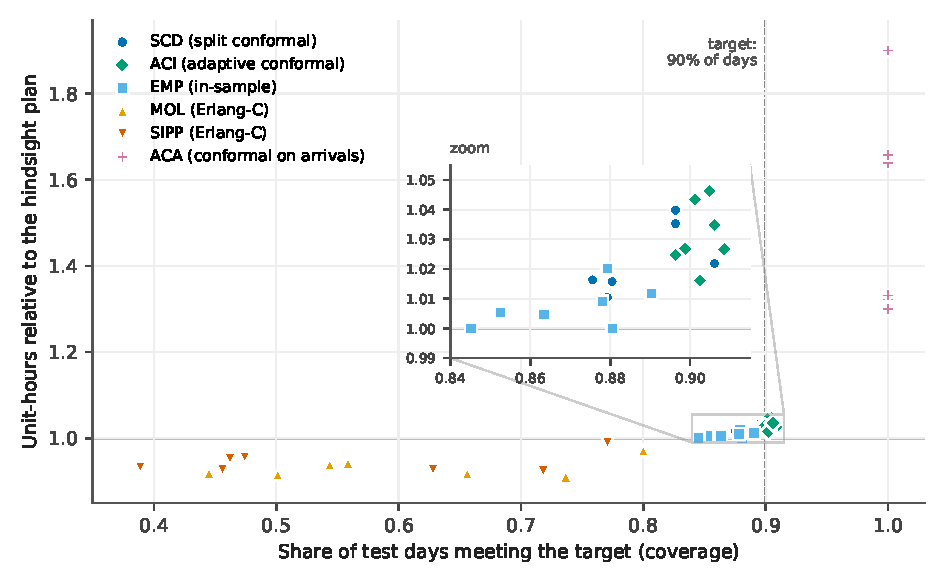
\includegraphics[width=0.92\linewidth]{fig_coverage_cost.pdf}
\caption{Coverage and cost of each rule in each of the seven systems (primary configuration: 80 training days, 90\% target, at most 5\% of calls delayed). Cost is the median over planning dates of unit-hours relative to the hindsight plan. The inset enlarges the region near the target.}
\label{fig:cc}
\end{figure}

\begin{table}[t]
\centering
\caption{Coverage (share of test days meeting the target) by rule and system, primary configuration, with the moving-block bootstrap 95\% interval for SCD. Last column: SCD's unit-hours relative to the hindsight plan (median over planning dates).}
\label{tab:res}
\small
\setlength{\tabcolsep}{4pt}
\begin{tabular}{lccccccc}
\toprule
System & SCD [95\% CI] & ACI & EMP & MOL & SIPP & ACA & SCD cost \\
\midrule
NYC area Q4 & \res{covSCDArea} [\res{loSCDArea}, \res{hiSCDArea}] & \res{covACIArea} & \res{covEMPArea} & \res{covMOLArea} & \res{covSIPPArea} & \res{covACAArea} & \res{relSCDArea} \\
Staten Island & \res{covSCDSI} [\res{loSCDSI}, \res{hiSCDSI}] & \res{covACISI} & \res{covEMPSI} & \res{covMOLSI} & \res{covSIPPSI} & \res{covACASI} & \res{relSCDSI} \\
Bronx & \res{covSCDBX} [\res{loSCDBX}, \res{hiSCDBX}] & \res{covACIBX} & \res{covEMPBX} & \res{covMOLBX} & \res{covSIPPBX} & \res{covACABX} & \res{relSCDBX} \\
Manhattan & \res{covSCDMN} [\res{loSCDMN}, \res{hiSCDMN}] & \res{covACIMN} & \res{covEMPMN} & \res{covMOLMN} & \res{covSIPPMN} & \res{covACAMN} & \res{relSCDMN} \\
Queens & \res{covSCDQN} [\res{loSCDQN}, \res{hiSCDQN}] & \res{covACIQN} & \res{covEMPQN} & \res{covMOLQN} & \res{covSIPPQN} & \res{covACAQN} & \res{relSCDQN} \\
Brooklyn & \res{covSCDBK} [\res{loSCDBK}, \res{hiSCDBK}] & \res{covACIBK} & \res{covEMPBK} & \res{covMOLBK} & \res{covSIPPBK} & \res{covACABK} & \res{relSCDBK} \\
San Francisco & \res{covSCDSF} [\res{loSCDSF}, \res{hiSCDSF}] & \res{covACISF} & \res{covEMPSF} & \res{covMOLSF} & \res{covSIPPSF} & \res{covACASF} & \res{relSCDSF} \\
\bottomrule
\end{tabular}
\end{table}

\subsection{Pre-specified hypotheses}

\emph{H1 was not supported.} The lower 95\% bound of SCD's coverage was at least 0.85 in \res{hOneOk} of 7 systems, one short of the pre-specified six; it fell to \res{hOneLoBX} in the Bronx and \res{hOneLoQN} in Queens. The point estimates in those systems, \res{covSCDBX} and \res{covSCDQN}, were about two percentage points below the nominal 0.90.

\emph{H2 was not supported.} EMP's coverage was below SCD's in all \res{empBelowScd} systems (\res{covEMPMin} to \res{covEMPMax}), but the per-system one-sided tests gave $p=\res{hTwoPMin}$ to $\res{hTwoPMax}$, and none remained below 0.05 after Holm adjustment (smallest adjusted $p=\res{hTwoHolmMin}$).

\emph{H3 was supported} in all \res{hThreeSig} systems (largest Holm-adjusted $p=\res{hThreePMax}$).

\emph{H4 was supported.} Pooled over systems, SCD's window coverage fell as demand grew from the calibration days to the test window (Spearman $\rho=\res{hFourRho}$, one-sided permutation $p=\res{hFourP}$; Figure~\ref{fig:drift}a). In the \res{nLoadUp} windows whose demand was more than 3\% above the calibration days, SCD's mean coverage was \res{covLoadUp}; in the \res{nLoadDown} windows more than 3\% below, it was \res{covLoadDown}; within $\pm3\%$ (\res{nLoadFlat} windows) it was \res{covLoadFlat}.

\begin{figure}[t]
\centering
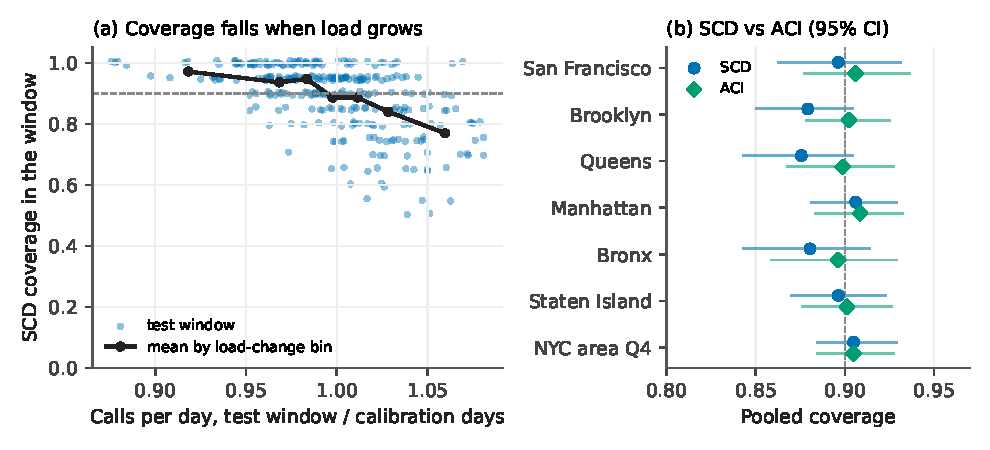
\includegraphics[width=\linewidth]{fig_drift.pdf}
\caption{Drift. (a) SCD coverage in each 20-day test window against the ratio of mean daily calls in the window to the calibration days (all seven systems; points jittered vertically by at most 0.008), with means within seven equal-count bins. (b) Pooled coverage of SCD and of the adaptive level (ACI, $\gamma=0.05$) in each system; the dashed line is the 90\% target.}
\label{fig:drift}
\end{figure}

\subsection{Adaptive level and the spread of window coverage}

Updating the level from one window to the next brought coverage to \res{covACIMin}--\res{covACIMax} in every system (Figure~\ref{fig:drift}b), at \res{relACIMin} to \res{relACIMax} times the hindsight unit-hours. The result did not depend on the step size: with $\gamma=0.02$ and $0.10$ coverage ranged from \res{gTwocovMin} to \res{gTencovMax}.

Window coverage varied more than exchangeability allows. Pooled over systems, the standard deviation of SCD's coverage across windows was \res{condSdObs}, against \res{condSdTh} under the exchangeable model, and \res{condBelowObs}\% of windows fell below 0.75, against \res{condBelowTh}\% expected. Successive weeks of EMS demand are not exchangeable, and the guarantee in equation~\eqref{eq:guarantee} holds on average over windows only to the extent that drift averages out.

\subsection{Secondary configurations}

The pattern held in every secondary configuration. With 40 training days SCD's coverage was \res{nFortycovSCDMin}--\res{nFortycovSCDMax} and ACI's \res{nFortycovACIMin}--\res{nFortycovACIMax}; with 160 days, \res{nOneSixtycovSCDMin}--\res{nOneSixtycovSCDMax} and \res{nOneSixtycovACIMin}--\res{nOneSixtycovACIMax}. At a 95\% target SCD reached \res{aFivecovSCDMin}--\res{aFivecovSCDMax} and ACI \res{aFivecovACIMin}--\res{aFivecovACIMax}, at \res{aFiverelSCDMin}--\res{aFiverelSCDMax} times the hindsight cost; at an 80\% target, \res{aTwentycovSCDMin}--\res{aTwentycovSCDMax} and \res{aTwentycovACIMin}--\res{aTwentycovACIMax}. With the 10-minute target SCD reached \res{tTencovSCDMin}--\res{tTencovSCDMax}, ACI \res{tTencovACIMin}--\res{tTencovACIMax}, and MOL \res{tTencovMOLMin}--\res{tTencovMOLMax}. ACA cost \res{aFiverelACAMin} to \res{aFiverelACAMax} times the hindsight plan at the 95\% target. In the primary configuration no conformal or in-sample rule reached the top of the $\theta$ grid (\res{flagsAll} flagged cases).

\section{Discussion}

Across seven EMS systems and more than three years of out-of-sample planning, calibrating the staffing decision on recent days gave plans that met a nine-days-in-ten service target close to the promised rate, at a cost a few percent above the best plan chosen in hindsight. The rules in common use did not deliver this promise: the Erlang-C rules met the day-level target on between four and eight days in ten, and they did so with fewer unit-hours, so their apparent economy is partly a lower level of service. Putting the conformal band around the demand forecast instead of the decision used \res{acaOverSCDMin}--\res{acaOverSCDMax}\% more unit-hours than SCD.

The result that matters most in practice is the one the pre-specified validity test did not quite pass. When demand grew after the calibration days, coverage fell, and in the Bronx, Queens and Brooklyn the pooled coverage was about two points short of nominal. This is what conformal theory predicts when exchangeability fails \citep{barber2023beyond}, and the remedy is cheap: adjusting the level according to how many recent days missed the target restored nominal coverage in every system for \res{aciOverSCDMin}--\res{aciOverSCDMax}\% more unit-hours than SCD.

The comparison with ACA carries a general lesson for decisions made under conformal guarantees. A decision needs its own outcome to be reliable, not every input to it. In staffing, a band that covers every hour of demand pays for hours that a queue would have absorbed. Calibrating the score of the decision itself (here, the safety factor a day needed) puts the guarantee where it is wanted and lets the queue's dynamics, captured by trace-driven simulation, decide what a busy hour costs. This is the reasoning behind conformal risk control \citep{angelopoulos2024conformal}; the present study shows its size on real operations data.

For an EMS agency the rule needs only what most agencies already hold: a few months of dispatch records with call times and unit busy times. The steps are: compute the hourly load from the older half of the window; for each recent day, find by simulation the smallest safety factor that would have met the target; take the appropriate rank of these factors; and staff by the square-root rule with that factor. Re-run before each planning period, and raise the level when more days than intended have recently missed the target. The code is available (see Data availability).

\subsection{Limitations}

The service model is a single pool without geography: it does not represent travel times, unit relocation, dispatch priorities, or the requirement that the nearest unit respond, so the delays here are waits for any free unit, not response times. Busy time stands in for the full unit commitment, including transport and hospital offload. Each day was simulated from an empty system at 04:00, ignoring calls carried over from the previous night. The plan family varies one safety factor across all hours; shift structures, breaks and minimum crew sizes were not modelled. Only weekdays were studied. Windows of 20 days are short, so the coverage of any one window is noisy, and the planning dates share calibration days, which the block bootstrap only partly accounts for. The data were prepared for an earlier study by the same author; the present analyses were specified and run afterwards and none were tuned on outcomes, but the author knew some features of the data (listed in the plan). Finally, the guarantee holds for the simulated system; it transfers to real operations only as far as the simulator reproduces them.

\section{Conclusions}

A staffing plan can carry an explicit reliability promise, such as meeting the service target on nine days in ten, by calibrating the decision on recent days rather than by trusting a queueing formula or calibrating the demand forecast. In seven EMS systems the promise was met nearly at the nominal rate for a few percent more unit-hours than hindsight allows. Where demand grows, the calibration level should adapt to recent misses.

\section*{Data availability}
The dispatch data are public \citep{nycems2026,sffire2026}. The analysis plan with its commit history, the code, the simulator and the result files are available at \repolink.

\ifdefined\ANON\else
\section*{CRediT authorship contribution statement}
\textbf{Thanh Van Nguyen:} Conceptualization, Methodology, Software, Formal analysis, Data curation, Writing -- original draft, Writing -- review \& editing.
\fi

\section*{Declaration of generative AI and AI-assisted technologies}
During the preparation of this work the author used Claude (Anthropic) to help design the analysis, write and test the code, search the literature and check every reference against Crossref and arXiv, and draft and edit the text. The author chose the research question, approved the analysis plan and its amendment before the analyses were run, and checked the results. After using this tool, the author reviewed and edited the content as needed and takes full responsibility for the content of the publication.

\section*{Ethics}
The study used only public, de-identified administrative records and involved no human participants; ethics review was not required.

\section*{Funding}
This research did not receive any specific grant from funding agencies in the public, commercial, or not-for-profit sectors.

\section*{Declaration of competing interest}
The author declares no known competing financial interests or personal relationships that could have appeared to influence the work reported in this paper.

\bibliographystyle{unsrtnat}
\bibliography{refs}

\end{document}
